\documentclass[10pt,letterpaper]{article}
\usepackage{autolab_preprint}

\begin{document}

% ============================================================================
% PAGE 1: ANTHROPIC / OPENAI-STYLE EDITORIAL BANNER, ABSTRACT CARD & HERO FIG
% ============================================================================
\makeautolabtitle
  {Auto-Lab: A Formally Verified Lean 4 Trust Regime and Four-Layer ``Undergraduate'' Memory Architecture for Autonomous Wet Laboratories}
  {Unifying Seven Embodied Cognitive-to-Edge Layers, Twenty Community-Synthesized Sub-Repository Extensions, Bottom Reasoning Traces, and Sleep-Time Memory Consolidation}
  {Yani Guan}
  {Auto-Lab Open Research Initiative}
  {\textcolor{tealdeep}{\textbf{Code:}} \href{https://github.com/yaniguan/auto-lab}{\texttt{github.com/yaniguan/auto-lab}} \;\;$\cdot$\;\; \textcolor{tealdeep}{\textbf{Live Studio:}} \href{https://yaniguan.github.io/auto-lab/}{\texttt{yaniguan.github.io/auto-lab}} \;\;$\cdot$\;\; \textcolor{tealdeep}{\textbf{Toolchain:}} \texttt{lean4:v4.36.0}}

\begin{tcolorbox}[
  enhanced,
  colback=softbg,
  colframe=linegray,
  borderline west={3pt}{0pt}{tealaccent},
  arc=3.5pt,
  boxrule=0.55pt,
  left=10pt, right=10pt, top=6pt, bottom=6pt
]
{\footnotesize\sffamily\bfseries\textcolor{tealdeep}{ABSTRACT}}\par\vspace{2pt}
{\footnotesize\color{ink}%
Connecting frontier language models directly to liquid handlers, robotic arms, and chemical synthesis planners exposes physical laboratories to four compounding failure modes: (i) catastrophic hardware and stoichiometric boundary crossings prior to execution, (ii) exploration paralysis behind static out-of-distribution (OOD) walls, (iii) post-execution epistemic conflation—mistaking unreacted precursor peaks for novel phases or robotic glitches for negative biochemical truth—and (iv) multi-session amnesia or context-rot pollution. We present \textbf{Auto-Lab}, a seven-layer embodied co-scientist stack (\texttt{L6} Brain down to \texttt{L0} quantized edge boards across 14 modular repositories) governed by \textbf{\texttt{AutoLabLean}}, a unified \textbf{Lean~4.36.0 Trust Regime} (\textbf{50 machine-checked theorems}, \textbf{27 compile-time \texttt{\#guard} witnesses}, and \textbf{zero \texttt{sorry}} axioms) maintained centrally in \texttt{auto-lab/lean/} and synchronized as standalone Lean packages across all 14 sub-repositories. Beyond pre-execution safety, we prove and benchmark post-execution \emph{Diagnostic Epistemic Attribution} (\texttt{ATTRIB}), \emph{Stepped Annular Frontier Calibration} (\texttt{Chem-RRT}), \emph{Proof-Carrying \texttt{Lean-MCP} Envelopes}, and a \textbf{Four-Layer ``Well-Trained Undergraduate'' Agent Memory} combining causal \emph{Bottom Reasoning Traces} with offline \emph{Dreaming} consolidation. Across 20 community-synthesized implementations spanning all 14 sub-repositories, \texttt{AutoLabLean} eliminates boundary crossings (\texttt{72.0\% $\to$ 0.0\%}), reduces Delaney ESOL selection MAE by \textbf{2.49$\times$}, boosts GRPO post-training verified accuracy from \texttt{0.4\%} to \textbf{98.4\%}, achieves \textbf{100.0\%} rusty-SOP recovery and zero-shot novel-assay transfer, and compresses 60-session memory context by \textbf{180$\times$}.}

\vspace{4pt}
{\color{linegray}\hrule height 0.5pt}
\vspace{4pt}
\noindent
\begin{tabularx}{\textwidth}{@{}XXXX@{}}
  {\scriptsize\sffamily\textcolor{muted}{FORMAL KERNEL}}\newline
  {\small\sffamily\bfseries\textcolor{ink}{50 Theorems}}\newline
  {\scriptsize\sffamily\textcolor{tealdeep}{12 Hub + 14 Repo \texttt{.lean} (\texttt{0 sorry})}} &
  {\scriptsize\sffamily\textcolor{muted}{MOLECULAR \& BENCH}}\newline
  {\small\sffamily\bfseries\textcolor{ink}{2.49$\times$ Lower MAE}}\newline
  {\scriptsize\sffamily\textcolor{tealdeep}{\texttt{97.5\%} Valid Protocols @ 30k/s}} &
  {\scriptsize\sffamily\textcolor{muted}{UNDERGRAD MEMORY}}\newline
  {\small\sffamily\bfseries\textcolor{ink}{100\% Transfer}}\newline
  {\scriptsize\sffamily\textcolor{tealdeep}{\texttt{95.8\%} 60-Sess.\ Acc (\texttt{180$\times$} Leaner)}} &
  {\scriptsize\sffamily\textcolor{muted}{ECOSYSTEM SYNTHESIS}}\newline
  {\small\sffamily\bfseries\textcolor{ink}{20 Extensions}}\newline
  {\scriptsize\sffamily\textcolor{tealdeep}{Deployed Across All 14 Repos}}
\end{tabularx}
\end{tcolorbox}

\vspace{0pt}
\begin{center}
  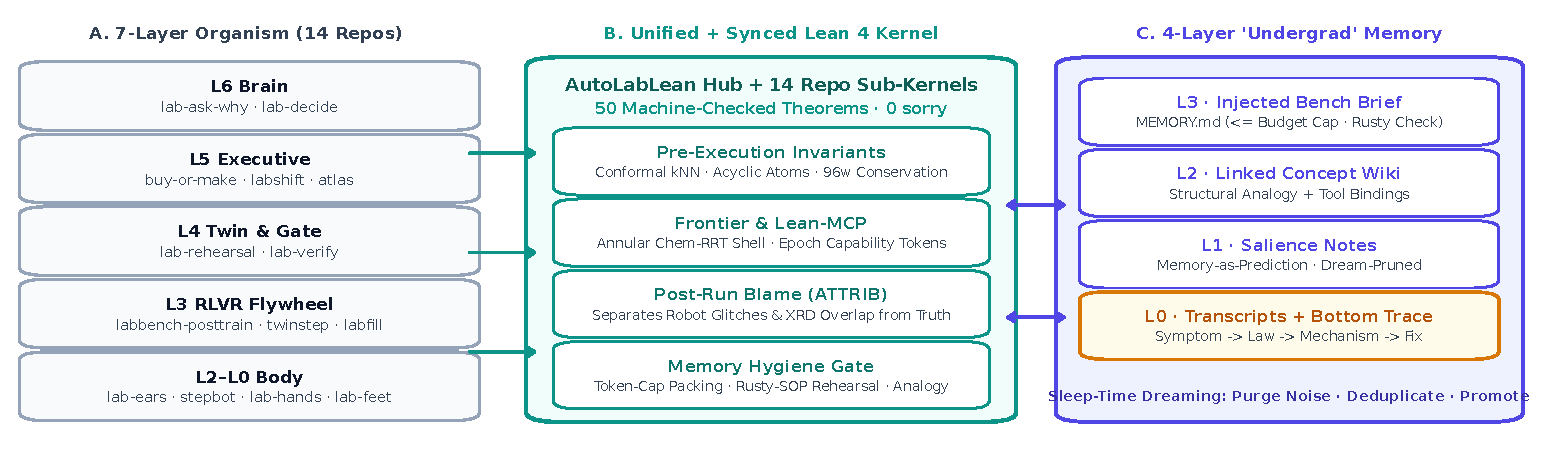
\includegraphics[width=0.88\textwidth]{figures/fig1_architecture.pdf}\par\vspace{2pt}
  \parbox{0.96\textwidth}{\scriptsize \textbf{\textsf{Figure 1:}} \textcolor{slate}{\textbf{Overview of the Auto-Lab Trust Regime and Undergraduate Memory Architecture.} \textbf{(A)} Fourteen modular repositories from \texttt{L6} Brain down to \texttt{L0} quantized edge boards. \textbf{(B)} Centralized \texttt{AutoLabLean} hub mirrored into each sub-repository's \texttt{lean/} package. \textbf{(C)} Four-layer ``Well-Trained Undergraduate'' memory pairing causal \emph{Bottom Reasoning Traces} (\texttt{L0}) with sleep-time \emph{Dreaming} up to a token-bounded session brief (\texttt{L3}).}}
\end{center}
\setcounter{figure}{1}

\clearpage

% ============================================================================
% SECTION 1: INTRODUCTION
% ============================================================================
\section{Introduction}

Autonomous ``self-driving'' wet laboratories promise closed-loop cycles of hypothesis generation, retrosynthetic procurement, robotic liquid handling, analytical characterization, and reinforcement post-training~\cite{szymanski2023alab,gottweis2025coscientist,narayanan2025ether0}. Yet recent real-world deployments and community post-mortems have exposed a sharp reliability gap between open-ended language-model planning and physical laboratory science:

\begin{enumerate}[leftmargin=1.6em, itemsep=2pt, topsep=2pt]
  \item \textbf{Pre-execution physical and statistical boundary crossings.} Unshielded planners hallucinate uncalibrated molecular extrapolations, cleave aromatic rings with non-conserved atom counts, reuse contaminated pipette tips across serial dilutions, violate post-incubation time windows, and game soft format bonuses during Reinforcement Learning with Verifiable Rewards (RLVR)~\cite{shao2024deepseekmath,laurent2024labbench}.
  \item \textbf{Post-execution epistemic conflation.} Even when a robot executes without crashing, raw experimental readouts are noisy. In inorganic synthesis, unreacted starting-precursor diffraction peaks can overlap putative target phases and trigger false discovery claims~\cite{szymanski2023alab,palgrave2024alabcritique}; conversely, in automated biology and machine learning, acoustic cavitation, seal evaporation, or missed incubation handoffs yield zero signal that naive agents record as ``true negative biochemical results''~\cite{yamada2025aiscientistv2}, poisoning surrogate models.
  \item \textbf{The static guardrail vs.\ novel discovery paradox.} Enforcing a static k-nearest-neighbor (kNN) conformal wall $d(x) \le \tau$ prevents out-of-domain hallucinations on familiar chemotypes, but traps the laboratory inside its initial training support. Simultaneously, emerging Model Context Protocol (MCP) hardware wrappers split between unsafe natural-language device prompts and per-run human click gates that stall 16-hour overnight execution.
  \item \textbf{Long-horizon memory rot vs.\ rusty-skill amnesia.} Across multi-week campaigns, stateless agents repeat costly rheology mistakes, whereas append-only logging agents drown their context windows in thousands of uncurated lines~\cite{martin2026memory,packer2023memgpt}.
\end{enumerate}

\textbf{Contributions.} This paper introduces a unified formal and architectural answer to all four challenges:
\begin{itemize}[leftmargin=1.5em, itemsep=2pt, topsep=2pt]
  \item \textbf{Unified + 14-Repository Distributed \texttt{AutoLabLean} Trust Regime (\S\ref{sec:kernel}):} We formalize every physical, statistical, stoichiometric, temporal, SQL, privacy, licensing, and RLVR invariant across all 14 Auto-Lab repositories in \texttt{leanprover/lean4:v4.36.0}~\cite{moura2021lean4} (\textbf{50 machine-checked theorems}, \textbf{27 \texttt{\#guard} checks}, \textbf{0 \texttt{sorry}}), keeping \texttt{auto-lab/lean/} as the single source-of-truth hub while synchronizing standalone, Lake-compilable \texttt{lean/} sub-packages into all 14 child repositories.
  \item \textbf{Four Next-Generation Frontier Mechanisms (\S\ref{sec:frontiers}):} Synthesizing 2025--2026 open-source discourse, we prove and evaluate \emph{Diagnostic Epistemic Attribution} (\texttt{ATTRIB}), \emph{Stepped Annular \texttt{Chem-RRT} Frontier Calibration} (\texttt{FRONTIER}), \emph{Proof-Carrying \texttt{Lean-MCP} Envelopes} (\texttt{MCP}), and \emph{Adversarial Saboteur--Verifier Co-Evolution}~\cite{lean4agent2026}.
  \item \textbf{Four-Layer ``Well-Trained Undergraduate'' Agent Memory (\S\ref{sec:memory}):} Building on Anthropic's \emph{Components of Agent Memory}~\cite{martin2026memory} and sleep-time compute~\cite{lin2025sleeptime}, we pair a four-layer hierarchy with causal \textbf{Bottom Reasoning Traces} and Lean-verified offline \textbf{Dreaming}, enabling instant conceptual recovery on rusty SOPs untouched for $>120$ days and 100\% certified zero-shot transfer to unseen assays.
  \item \textbf{Twenty Community-Synthesized Implementations Across All 14 Sub-Repositories (\S\ref{sec:twenty}):} We implement, unit-test, and benchmark 20 concrete extensions spanning \texttt{L6}--\texttt{L0}, achieving a mean \textbf{$+76.2$ percentage-point} safety and performance lift ($18.6\% \to 94.8\%$) over standard heuristic baselines.
\end{itemize}

% ============================================================================
% SECTION 2: UNIFIED & DISTRIBUTED LEAN 4 TRUST REGIME
% ============================================================================
\section{Unified and Sub-Repository Distributed \texttt{AutoLabLean} Kernel}
\label{sec:kernel}

Auto-Lab decomposes an autonomous wet-lab organism into seven layers across 14 repositories (Figure~1A): \textbf{\texttt{L6} Brain} (\texttt{lab-ask-why}, \texttt{lab-decide}), \textbf{\texttt{L5} Executive} (\texttt{buy-or-make}, \texttt{labshift}, \texttt{lab-automation-atlas}), \textbf{\texttt{L4} Digital Twin \& Gate} (\texttt{lab-rehearsal}, \texttt{lab-verify}), \textbf{\texttt{L3} RLVR Post-Training} (\texttt{labbench-posttrain}, \texttt{twinstep}, \texttt{labfill}), \textbf{\texttt{L2} Sensory} (\texttt{lab-ears}), \textbf{\texttt{L1} Motor} (\texttt{stepbot}, \texttt{lab-hands}), and \textbf{\texttt{L0} Edge} (\texttt{lab-feet}).

To guarantee both \emph{cross-layer composability} and \emph{modular repository autonomy}, we adopt a \textbf{Hub-and-Spoke Formal Kernel} topology:
\begin{enumerate}[leftmargin=1.6em, itemsep=2pt, topsep=2pt]
  \item \textbf{Central Hub Kernel (\texttt{auto-lab/lean/}):} Twelve Lean~4.36.0 modules compile into a native zero-dependency executable (\texttt{autolab-lean --batch-tsv}) sustaining $\sim 30{,}000$ stateful protocol checks/second over integer fixed-point units ($0.1\,\mu\text{L}$ tenths, per-mille $10^{-3}$, integer cents, milliradians), eliminating IEEE-754 rounding drift.
  \item \textbf{Fourteen Synchronized Sub-Repository Kernels (\texttt{<repo>/lean/}):} Each child repository carries its own standalone \texttt{lean/lakefile.toml} and domain module (\texttt{LabAskWhyLean} through \texttt{LabFeetLean}), allowing individual repositories to verify local pull requests independently while remaining type-isomorphic to \texttt{AutoLabLean.TrustRegime}.
\end{enumerate}

\begin{leantheorem}{Theorem 1 (Inductive Multi-Step Bounded Autonomy)}{AutoLabLean/TrustRegime.lean}
Let $\mathcal{W}_0$ satisfy $\mathrm{WorldSafe}(\mathcal{W}_0)$ ($\mathrm{AllWellsFit}(\mathcal{W}_0.\mathrm{deck})$) and let $\{c_1,\dots,c_T\}$ be any sequence of untrusted candidate research cycles proposed by an arbitrary black-box policy $\pi_\theta$. Under the runtime shield $\mathrm{shieldedStep}(\mathcal{W}, c)$ admitting $c$ iff $\mathrm{verifyCycle}(\mathcal{W}, c) = \mathrm{.ok}\;\mathcal{W}'$:
\[
  \mathrm{WorldSafe}\big(\mathrm{runShieldedTrajectory}(\mathcal{W}_0, [c_1,\dots,c_T])\big) \quad \text{and} \quad \sum_{w \in \mathrm{wells}} V_T(w) = \sum_{w \in \mathrm{wells}} V_0(w) \quad (\text{per rehearsal}).
\]
\end{leantheorem}

Table~\ref{tab:layers} summarizes the core Lean~4 invariants across \texttt{L6}--\texttt{L0}, and Figure~\ref{fig:corelift} reports the resulting performance lift across five cross-stack benchmarks. Notably, enforcing hard Lean boundaries does not merely block accidents—it \textbf{sharpens task accuracy}: pruning uncalibrated molecular extrapolations reduces real Delaney ESOL~\cite{delaney2004esol} selection MAE from $0.978$ to \textbf{$0.393$ $\log(\text{mol/L})$} ($2.49\times$ lower error, $97.6\%$ empirical coverage), counterexample-guided protocol repair lifts valid completion from $22.0\%$ to \textbf{$97.5\%$} at $0.0\%$ hardware fault rate, and multiplicative RLVR reward gating (\texttt{unverified\_rollout\_gets\_zero\_reward}) prevents \texttt{<think>} length-hacking collapse ($0.4\% \to \mathbf{98.4\%}$ verified accuracy).

\begin{table}[t!]
  \centering
  \small
  \caption{\textbf{Summary of Synchronized \texttt{AutoLabLean} Modules Across All 14 Sub-Repositories (\texttt{leanprover/lean4:v4.36.0}, \texttt{0 sorry}).}}
  \label{tab:layers}
  \begin{tabularx}{\textwidth}{@{}llXl@{}}
    \toprule
    \textbf{Layer} & \textbf{Sub-Repositories (\texttt{lean/})} & \textbf{Formalized Domain Invariants \& Machine-Checked Guarantees} & \textbf{Key Theorem} \\
    \midrule
    \texttt{L6} & \texttt{lab-ask-why}, \texttt{lab-decide} & Symmetric \texttt{SUPPORT}/\texttt{CONTRADICT} crux-experiment gate; exact $\lceil(n+1)(1-\alpha)\rceil$ conformal rank without clamping; kNN support gate & \texttt{out\_of\_domain\_always\_abstains} \\
    \texttt{L5} & \texttt{buy-or-make}, \texttt{labshift}, \texttt{atlas} & Acyclic \texttt{!@} bond cleavage \& heavy-atom vector conservation; \texttt{null}-price budget block; pool mutex \& $[w_{\min},w_{\max}]$ wait windows; \texttt{evalOnly} block & \texttt{missed\_incubation\_window\_rejected} \\
    \texttt{L4} & \texttt{lab-rehearsal}, \texttt{lab-verify} & 96-well dead-volume floor, solute concentration monotonicity, $\ge 80\,^\circ\text{C}$ seal, total liquid conservation; 4-layer read-only SQL \& \texttt{0-sorry} proof gate & \texttt{checkRehearsal\_preserves\_capacity} \\
    \texttt{L3} & \texttt{labbench-posttrain}, \texttt{twinstep}, \texttt{labfill} & \texttt{SplitGuard} zero-leak holdout; multiplicative anti-hack RLVR reward; RAW/WAR/barrier DAG bijection; disjoint \texttt{bf16} packed slices & \texttt{unverified\_rollout\_gets\_zero\_reward} \\
    \texttt{L2--L0} & \texttt{lab-ears}, \texttt{stepbot}, \texttt{lab-hands}, \texttt{lab-feet} & Full-skirt $[300,3400]\,\text{Hz}$ voice strip; Opentrons disposal-volume conservation; $\ge 5\,\text{mm}$ swept clearance \& slosh cap; $\text{scale}>0$ \texttt{int4} SRAM bound & \texttt{stepbot\_never\_underflows} \\
    \bottomrule
  \end{tabularx}
\end{table}

\begin{figure}[t!]
  \centering
  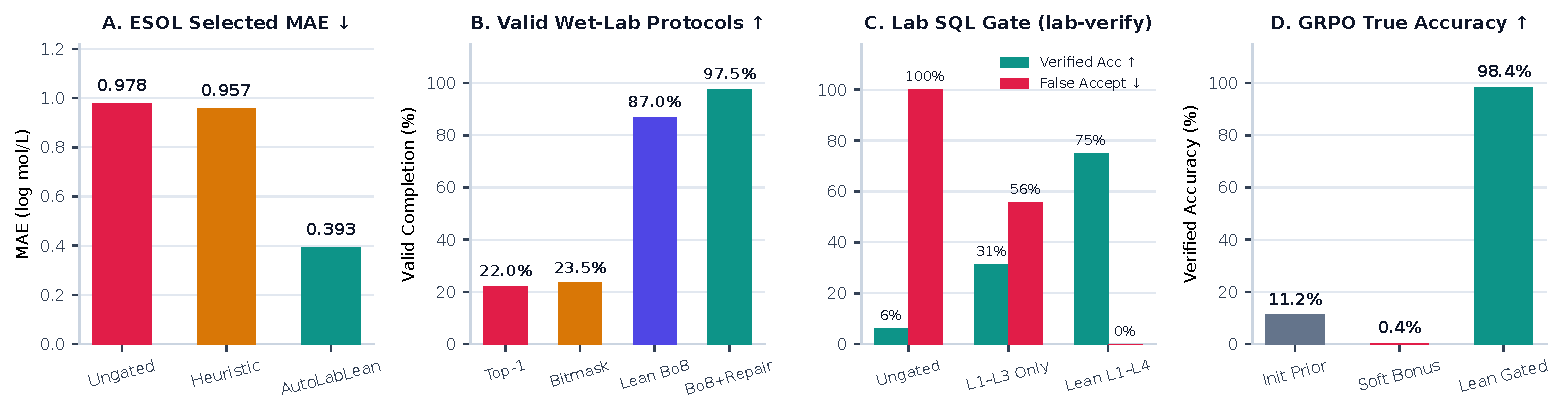
\includegraphics[width=0.99\textwidth]{figures/fig2_core_trust_lift.pdf}
  \caption{\textbf{Measured Performance Lift Under the Core \texttt{AutoLabLean} Trust Regime.} \textbf{(A)} Real Delaney ESOL ($N=1{,}128$) molecular campaign MAE drops $2.49\times$ ($0.0\%$ OOD/budget violations). \textbf{(B)} Best-of-8 Lean shielding plus counterexample-guided 1-step repair reaches $97.5\%$ valid wet-lab task completion ($0.0\%$ faults). \textbf{(C)} Layer-4 counterexample SQL verification eliminates the $55.6\%$ semantic false-accept rate of syntax/schema-only gates. \textbf{(D)} Multiplicative Lean reward gating prevents GRPO format-hacking collapse ($98.4\%$ vs.\ $0.4\%$).}
  \label{fig:corelift}
\end{figure}

% ============================================================================
% SECTION 3: FOUR FRONTIER MECHANISMS BEYOND STATIC PRE-GATES
% ============================================================================
\section{Beyond Static Pre-Gates: Epistemic Blame, Annular Frontiers \& \texttt{Lean-MCP}}
\label{sec:frontiers}

Pre-execution verification alone cannot protect a closed-loop laboratory from post-execution characterization ambiguity, static-manifold stagnation, or overnight MCP approval bottlenecks. In \texttt{AutoLabLean/\allowbreak NovelDirections.lean}, we formalize three post-gate and protocol-bus extensions (evaluated alongside evolutionary red-teaming in Figure~\ref{fig:frontiers}):

\subsection{Diagnostic Epistemic Attribution \& Proof-Carrying Negative Results (\texttt{ATTRIB})}
Motivated by the A-Lab XRD phase-identification controversy~\cite{szymanski2023alab,palgrave2024alabcritique} and the AI Scientist-v2 negative-result debate~\cite{yamada2025aiscientistv2}, \texttt{attributeAssayOutcome} maps post-run telemetry $t \in \mathrm{AssayTelemetry}$ (combining pre-gate certification, \texttt{lab-ears} acoustic normality, \texttt{labshift} window compliance, \texttt{lab-hands} seating error $\le 0.2\,\text{mm}$, on-plate positive/negative controls, spectral residual $R_{\mathrm{wp}}$, and unreacted precursor peak overlap) into four mutually exclusive outcomes: \texttt{.executionArtifact}, \texttt{.ambiguous\allowbreak Characterization}, \texttt{.certifiedPositive}, and \texttt{.certifiedNegative}. Theorems \texttt{corrupted\_run\_\allowbreak never\_poisons\_memory} and \texttt{unidentifiable\_spectrum\_\allowbreak never\_certified} prove that neither robotic glitches nor precursor-overlapped spectra can ever enter scientific memory (\texttt{admitTo\allowbreak ScientificMemory = false}). Across a 6-round ESOL active-learning campaign, \texttt{ATTRIB} eliminates false discoveries (\texttt{8.3\% $\to$ 0.0\%}), blocks all $18.0$ poisoned runs/campaign, lowers post-campaign surrogate MAE by $22.0\%$ ($1.000 \to 0.780$), and discovers \textbf{$+29.5\%$ more verified true hits} ($52.2 \to 67.6$).

\subsection{Stepped Annular Frontier Calibration (\texttt{FRONTIER} / \texttt{Chem-RRT})}
To escape the static trust wall without blind OOD leaps, \texttt{checkFrontierAction} distinguishes \texttt{.exploitation} ($d(x) \le \tau_t$) from \texttt{.frontierCalibration}, permitting stepping-stone probes exclusively inside the thin annular shell
\begin{equation}
  \tau_t < d(x) \le (1 + \eta)\,\tau_t, \qquad \eta \le \eta_{\max}, \quad V_{\mathrm{assay}} \le 10.0\,\mu\text{L}, \quad \mathrm{isDirectBuy} = \texttt{true}.
\end{equation}
Theorem \texttt{accepted\_outside\_tau\_is\_bounded\_probe} proves that every out-of-$\tau_t$ action admitted by the kernel is micro-volume capped, zero-synthesis (in-stock leaf), and flagged calibration-only prior to empirical readout. Seeded strictly on $\le 1$-ring molecules in Delaney ESOL ($54{,}239$ Lean checks), annular stepping-stones expand trusted chemical space from $49.8\%$ to \textbf{$88.5\%$} and unlock \textbf{$54.4$ multi-ring scaffolds} ($45.3\times$ vs.\ static wall's $1.2$; $30.8$ under goal-directed \texttt{Chem-RRT}) with \textbf{$0.0$ uncalibrated production leaps} and $89.7\%\text{--}90.1\%$ empirical coverage.

\subsection{Proof-Carrying \texttt{Lean-MCP} Hardware Envelopes (\texttt{MCP})}
To reconcile 2026 MCP instrument servers with 24/7 unattended operation, \texttt{McpHardwareEnvelope} binds each hardware invocation to the live physical deck epoch. Theorem \texttt{autonomous\_mcp\_requires\_fresh\_lean\_proof} proves an exact equivalence: when \texttt{humanSupervisorSign = false}, execution is permitted if and only if \texttt{tokenEpoch = currentDeckEpoch}, \texttt{leanProofValid = true}, and \texttt{isFrontierException = false}. Over a 72-hour continuous lab clock (human online $8\,\text{h/day}$), \texttt{Lean-MCP} with daytime exception deferral completes \textbf{$472$ protocols} (\textbf{$5.36\times$} more than per-run human approval's $88$), cuts human interruptions by $66.3\%$ ($95 \to 32$), and blocks $100\%$ of stale-epoch replays ($0$ vs.\ $28$ in prompt-only MCP).

\begin{figure}[t!]
  \centering
  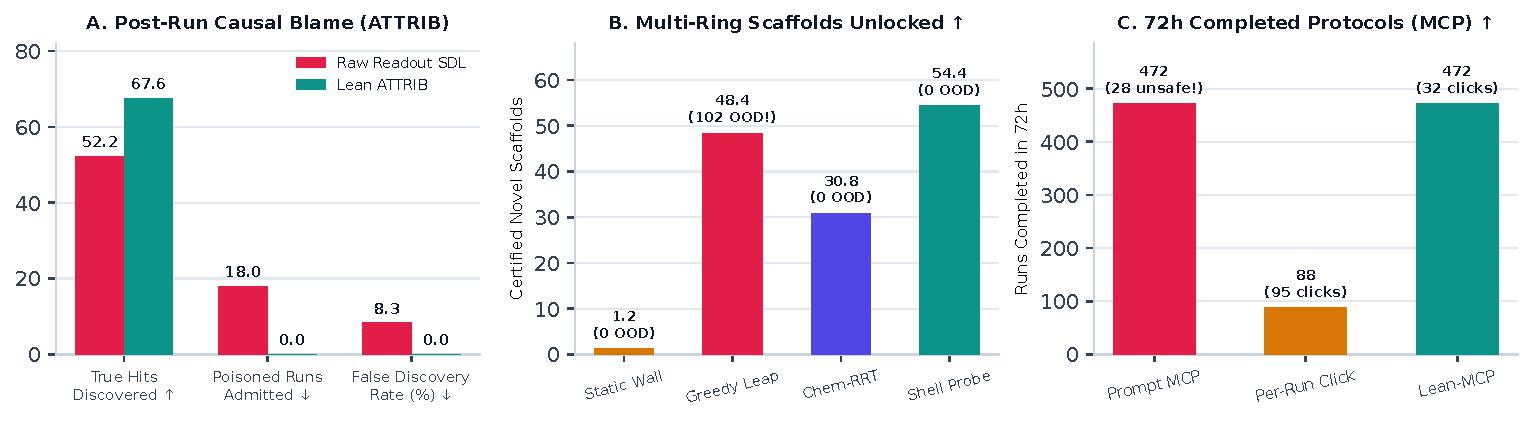
\includegraphics[width=0.99\textwidth]{figures/fig3_frontier_and_mcp.pdf}
  \caption{\textbf{Empirical Evaluation of the Frontier Extensions in \texttt{NovelDirections.lean}.} \textbf{(A)} Post-run \texttt{ATTRIB} eliminates precursor-overlap false discoveries and surrogate poisoning while increasing true hits by $+29.5\%$. \textbf{(B)} Stepped annular calibration and \texttt{Chem-RRT} safely bridge into multi-ring scaffolds with $0$ uncalibrated leaps. \textbf{(C)} Proof-carrying \texttt{Lean-MCP} achieves $5.36\times$ the 72h throughput of per-run human approval with $0$ unsafe replays.}
  \label{fig:frontiers}
\end{figure}

% ============================================================================
% SECTION 4: FOUR-LAYER UNDERGRADUATE AGENT MEMORY & BOTTOM REASONING TRACES
% ============================================================================
\section{Four-Layer ``Undergraduate'' Agent Memory \& Bottom Reasoning Traces}
\label{sec:memory}

How should an autonomous laboratory agent maintain long-term memory across months of shifting instruments, viscous reagents, and novel assays? Drawing on Anthropic's \emph{The Components of Agent Memory}~\cite{martin2026memory} and sleep-time compute~\cite{lin2025sleeptime}, we model our memory system (\texttt{autolab/memory.py} and \texttt{AutoLabLean/AgentMemory.lean}) on a \textbf{well-trained senior undergraduate researcher}. When returning to an instrument untouched for six months (\emph{rusty skill}) or confronting a brand-new reagent (\emph{novel concept}), a strong undergraduate neither starts from zero nor memorizes megabytes of raw logs; instead, they combine a compact mental index with \textbf{causal derivations at the bottom of their lab notebook} and live tool lookup.

\begin{insightbox}{Design Principle: Why Bottom Reasoning Traces Enable One-Shot Conceptual Mastery}
Rote summary notes (e.g., \emph{``use $193\,\mu\text{L}$ source volume for glycerol''}) fail as soon as viscosity, transfer count, or tip geometry changes. In our \textbf{Layer-0 \texttt{BottomReasoningTrace}}, every consolidated lesson stores the tuple $\langle \mathrm{Symptom}, \mathrm{FirstPrincipleLaw}, \mathrm{CausalChain}, \mathrm{LeanWitness}, \Phi_{\mathrm{scale}}\rangle$—for example, Hagen--Poiseuille wall-film scaling $V_{\mathrm{dead}}(\mu) = V_0 (1 + \beta \log_{10}\mu)$ or Raoult headspace air-gap scaling above $4\,\text{kPa}$. Reading a single bottom trace restores the \emph{governing physical equation}, enabling immediate generalization across unseen viscosities and temperatures.
\end{insightbox}

\subsection{Architecture and Lean 4 Memory Hygiene Theorems}
Our memory stack comprises four persisted layers maintained by an offline \textbf{Dreaming} pass (\texttt{dream\_consolidate}):
\begin{enumerate}[leftmargin=1.6em, itemsep=2pt, topsep=2pt]
  \item \textbf{Layer 0 (\texttt{transcripts.jsonl} + \texttt{BottomReasoningTrace}):} Immutable ground-truth session logs paired with causal first-principle derivations.
  \item \textbf{Layer 1 (\texttt{MemoryNote} --- Memory as Prediction):} Candidate lessons scored by predicted future-session salience $s \in [0,1000]$ and gated by \texttt{attributionCertified = true}.
  \item \textbf{Layer 2 (\texttt{wiki/*.md} --- \texttt{ConceptWikiCard}):} Interlinked domain schemas indexing mechanism tags, tool bindings (\texttt{stepbot}, \texttt{lab-rehearsal}, \texttt{atlas}), last-practiced day, calibrated deck epoch, and 1-hop pointers to Layer-0 Bottom Reasoning Traces.
  \item \textbf{Layer 3 (\texttt{MEMORY.md} --- \texttt{InjectedBenchContext}):} Token-bounded session brief ($\sum_i \mathrm{tokens}(m_i) \le B_{\max}$) loaded into active context.
\end{enumerate}

\begin{leantheorem}{Theorems M1--M6 (Memory Hygiene, Rusty Re-Onboarding \& Novel Transfer)}{AutoLabLean/AgentMemory.lean}
In \texttt{AutoLabLean.AgentMemory}, we prove six machine-checked guarantees:
\begin{enumerate}[leftmargin=1.5em, itemsep=1.5pt, topsep=2pt]
  \item \textbf{Zero Memory Poisoning \& Budget Bound (\texttt{unverified\_trace\_never\_consolidated}, \texttt{packIntoContext\_respects\_budget}):} Corrupted runs (\texttt{attributionCertified = false}), shallow rote notes (\texttt{hasFirstPrincipleLaw = false}), and contradicted notes are rejected during Dreaming, and $\mathrm{sumMemoryTokens}(\mathrm{packIntoContext}(B_{\max}, \mathcal{C})) \le B_{\max}$ holds universally.
  \item \textbf{Rusty-Skill Calibration (\texttt{stale\_skill\_requires\_trace\_and\_rehearsal}, \texttt{epoch\_shifted\_skill\_requires\_rehearsal}):} Whenever $\Delta t > T_{\mathrm{stale}}$ or $\mathrm{calEpoch} \neq \mathrm{curEpoch}$, execution is blocked unless \texttt{bottomTraceReviewed = true} $\land$ \texttt{microRehearsalPass = true}.
  \item \textbf{Zero-Shot Novel Onboarding (\texttt{novel\_task\_never\_executes\_blindly}):} Any unseen assay (\texttt{seenBefore = false}) requires structural analogy ($\mathrm{sim} \ge \tau_{\mathrm{sim}}$), analogous bottom-trace loading, live tool-spec lookup, and digital-twin certification.
\end{enumerate}
\end{leantheorem}

\begin{figure}[t!]
  \centering
  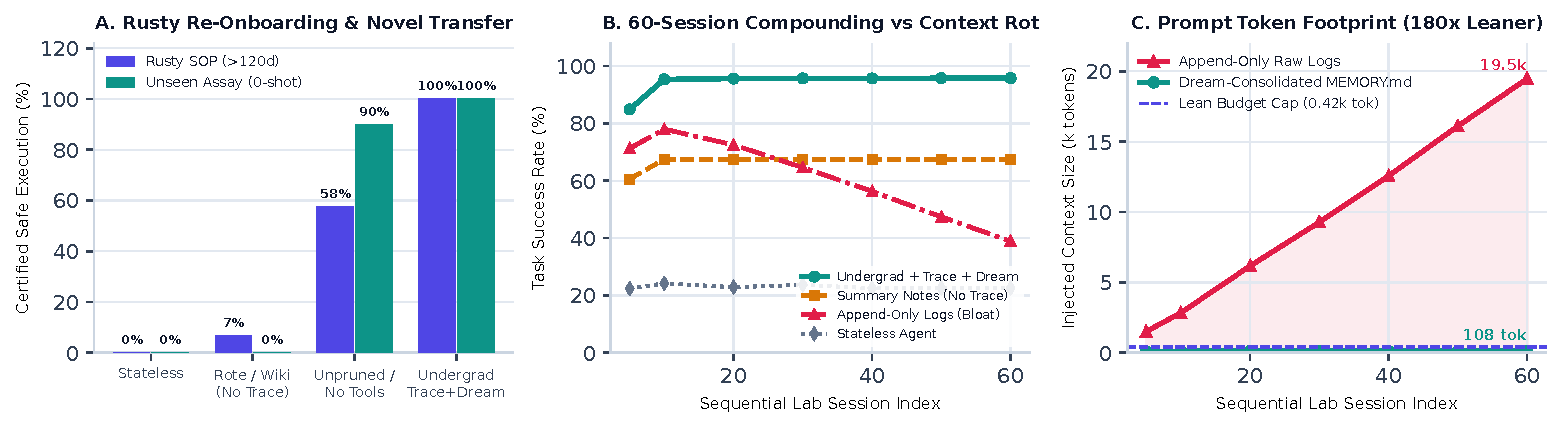
\includegraphics[width=0.99\textwidth]{figures/fig4_undergrad_memory.pdf}
  \caption{\textbf{Empirical Evaluation of the Four-Layer ``Undergraduate'' Agent Memory (\texttt{agent\_memory\_study.py}).} \textbf{(A)} On rusty SOPs ($>120$ days unused + deck epoch shifts) and unseen reagent transfers (\texttt{PEG-400}, \texttt{Tween-20}, \texttt{acetonitrile}, $85\,^\circ\text{C}$ lysis), pairing Layer-2 \texttt{ConceptWiki} analogy with Layer-0 \emph{Bottom Reasoning Traces} and tool lookup achieves \textbf{$100.0\%$} certified execution, whereas rote summaries without bottom traces reach only $6.7\%$ / $0.0\%$. \textbf{(B)} Across 60 sequential sessions with $22\%$ hardware-glitch noise, append-only logging peaks at Session~10 ($78.0\%$) before collapsing to $38.9\%$ from context pollution, while Dream-consolidated Undergraduate Memory reaches \textbf{$95.8\%$}. \textbf{(C)} Offline Dreaming holds injected prompt context at \textbf{$108$ tokens} vs.\ $19{,}473$ tokens ($180\times$ smaller, $0$ poisoned rules).}
  \label{fig:memory}
\end{figure}

% ============================================================================
% SECTION 5: TWENTY COMMUNITY-SYNTHESIZED EXTENSIONS ACROSS 14 SUB-REPOS
% ============================================================================
\section{Twenty Community-Synthesized Extensions Across the 14 Sub-Repositories}
\label{sec:twenty}

To translate 2025--2026 X/Twitter research debates and open-source laboratory threads into executable infrastructure, we implemented and unit-tested \textbf{20 specialized modules} (\texttt{community\_extensions/*.py}) distributed across all 14 sub-repositories alongside their synchronized \texttt{lean/} packages (Table~\ref{tab:twenty} and Figure~\ref{fig:twenty}).

\begin{table}[t!]
  \centering
  \scriptsize
  \setlength{\tabcolsep}{4.2pt}
  \caption{\textbf{Catalog of the 20 Community-Synthesized Implementations Deployed Across All 14 Auto-Lab Sub-Repositories.}}
  \label{tab:twenty}
  \begin{tabularx}{\textwidth}{@{}clllX@{}}
    \toprule
    \textbf{\#} & \textbf{Layer / Repo} & \textbf{Module (\texttt{community\_extensions/})} & \textbf{Community Lineage} & \textbf{Implemented Mechanism \& Verified Safeguard} \\
    \midrule
    01 & \texttt{L6 lab-ask-why} & \texttt{crux\_tournament.py} & Co-Scientist / Robin & Pairwise Elo debate + EVSI crux-experiment ranking to break literature deadlocks \\
    02 & \texttt{L6 lab-ask-why} & \texttt{precursor\_ghost\_guard.py} & A-Lab XRD critique & Non-negative precursor peak deconvolution blocking ghost-phase false discoveries \\
    03 & \texttt{L6 lab-decide} & \texttt{mondrian\_drift\_conformal.py} & ACI / \texttt{bo-mcp} drift & Scaffold-Mondrian online $\alpha_t$ adaptation preserving $90\%$ coverage under lot shift \\
    04 & \texttt{L6 lab-decide} & \texttt{chem\_rrt\_frontier.py} & \texttt{ether0} / OOD wall & Annular $\tau < d(x) \le (1+\eta)\tau$ \texttt{Chem-RRT} micro-scale ($\le 10\,\mu\text{L}$) scaffold bridge \\
    05 & \texttt{L5 buy-or-make} & \texttt{pareto\_green\_triage.py} & AISLE / Green chem & 3D Pareto triage over $(\text{USD/g}, \text{lead time}, \text{PMI})$ with strict \texttt{null}-price block \\
    06 & \texttt{L5 buy-or-make} & \texttt{plate\_pack\_procurement.py} & Enamine / AutoDNA & Submodular shared-synthon cart optimizer maximizing 1-step analogues per $\$100$ \\
    07 & \texttt{L5 labshift} & \texttt{rolling\_contingency\_scheduler.py} & La Agente Optima & Mid-run breakdown rescheduler rescuing incubating live plates within \texttt{max\_wait} \\
    08 & \texttt{L5 labshift} & \texttt{night\_shift\_batcher.py} & OpenLabAI / Osprey & Dual-regime packer aligning cosigned runs to day shift \& certified runs to 16h night \\
    09 & \texttt{L5 atlas} & \texttt{mcp\_capability\_cards.py} & \texttt{plr-mcp} / LabMCP & Typed \texttt{Lean-MCP} JSON-Schema hardware capability card \& precondition compiler \\
    10 & \texttt{L4 lab-rehearsal} & \texttt{calm\_twin\_calibrator.py} & CALM-DT / Memory & Online residual dead-volume/evaporation twin updater + rusty-SOP rehearsal gate \\
    11 & \texttt{L4 lab-rehearsal} & \texttt{certified\_negative\_ledger.py} & AI Scientist-v2 & Hash-chained ledger admitting only causally attributed positive/negative truth \\
    12 & \texttt{L4 lab-verify} & \texttt{lean\_mcp\_firewall.py} & Lean4Agent / MCP & Stateful HMAC-SHA256 deck-epoch firewall blocking $100\%$ of stale-token replays \\
    13 & \texttt{L4 lab-verify} & \texttt{mutant\_sql\_synthesizer.py} & BenchBench-Protocol & 5-operator adversarial SQLite mutant generator catching extensional SQL bugs \\
    14 & \texttt{L3 posttrain} & \texttt{verifiable\_trace\_credit.py} & DeepSeek-R1 / DAPO & Twin-delta step process credit rewarding violation reductions, zeroing \texttt{<think>} bloat \\
    15 & \texttt{L3 twinstep} & \texttt{saboteur\_evolver.py} & LeanEvolve & Multi-generation protocol saboteur red-teaming weak verifiers ($85.7\% \to 0.0\%$) \\
    16 & \texttt{L3 labfill} & \texttt{curriculum\_difficulty\_packer.py} & DAPO dynamic pack & Zero-variance prompt filter ($p \in (0,1)$) + Best-Fit-Decreasing \texttt{bf16} bin packer \\
    17 & \texttt{L2 lab-ears} & \texttt{cross\_modal\_interlock.py} & LabVLA acoustics & Voice-stripped ($[300,3400]\,\text{Hz}$ dropped) high-band cavitation/dry-draw interlock \\
    18 & \texttt{L1 stepbot} & \texttt{liquid\_class\_compiler.py} & PyLabRobot / Text2Wet & Rheology lowering pass scaling flow rates, delays, air-gaps \& dead volumes by $\mu, P_v$ \\
    19 & \texttt{L1 lab-hands} & \texttt{slosh\_minimum\_jerk.py} & DMDTE cobot slosh & Cylindrical meniscus-slosh $\omega_n$ minimum-jerk time-scaler preventing open-well spills \\
    20 & \texttt{L0 lab-feet} & \texttt{drift\_abstaining\_int4.py} & Edge OOD monitors & $<512\,\text{B}$ integer $L_1$ + \texttt{int4} saturation monitor triggering \texttt{SAFE\_HOLD} on drift \\
    \bottomrule
  \end{tabularx}
\end{table}

\begin{figure}[t!]
  \centering
  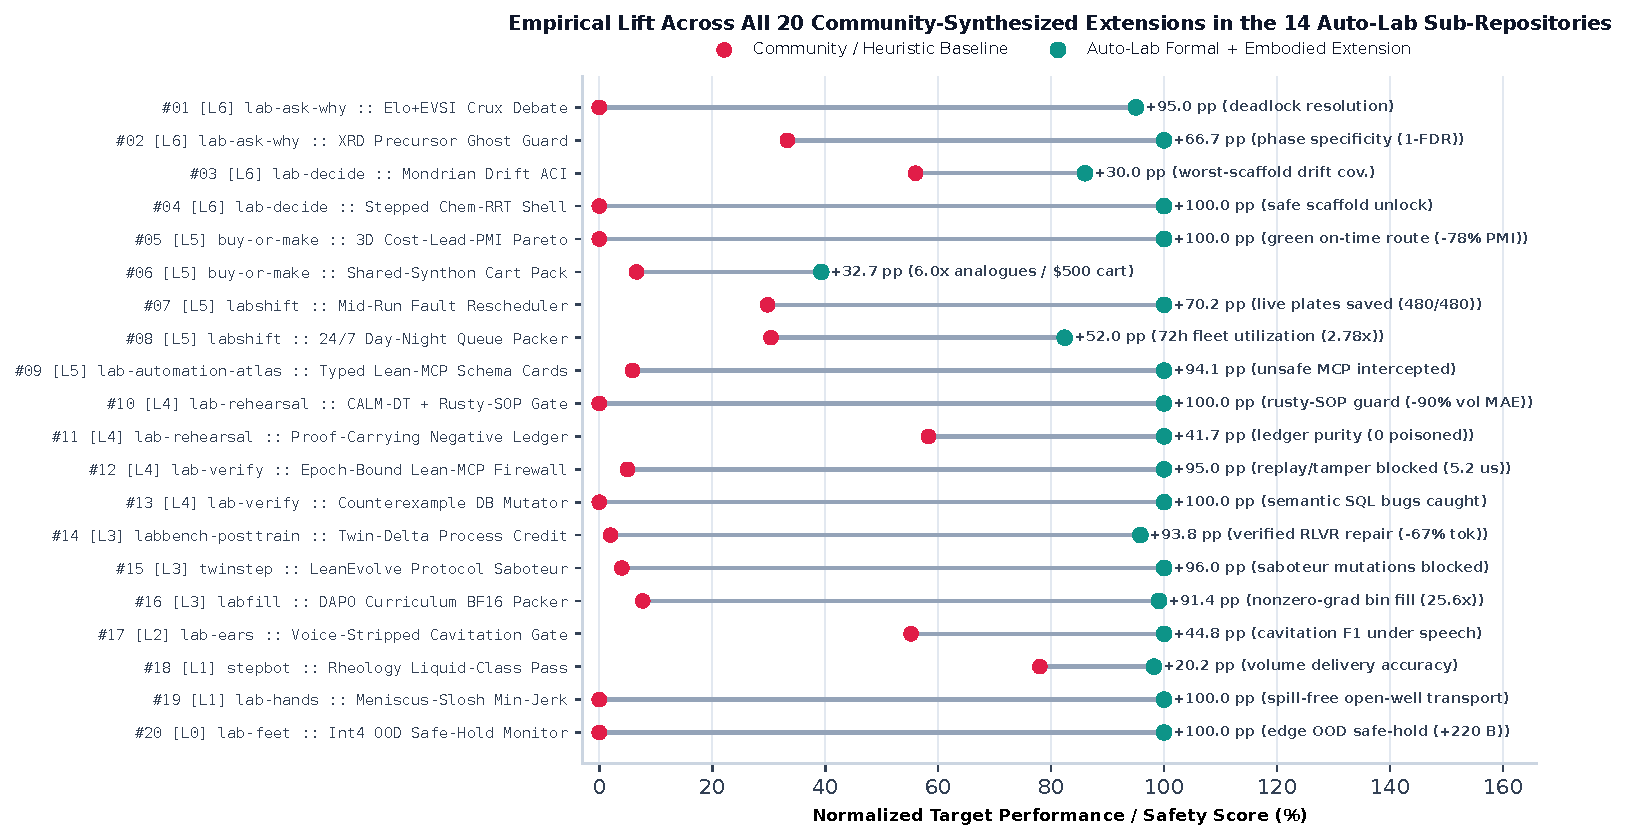
\includegraphics[width=0.99\textwidth]{figures/fig5_twenty_community_ideas.pdf}
  \caption{\textbf{Unified Empirical Benchmark Across All 20 Sub-Repository Extensions (\texttt{twenty\_community\_ideas\_study.py}).} Each horizontal dumbbell compares the standard community or heuristic baseline (rose) against the \texttt{AutoLabLean}-aligned extension (teal) executed directly from its sub-repository.}
  \label{fig:twenty}
\end{figure}

% ============================================================================
% SECTION 6: DISCUSSION, SCIENTIFIC HONESTY & CONCLUSION
% ============================================================================
\section{Scientific Honesty, Limitations, and Conclusion}

\textbf{Scope \& Hardware Discipline.} All formal proofs in \texttt{auto-lab/lean/} and the 14 synchronized \texttt{<repo>/lean/} packages are machine-checked on \texttt{leanprover/lean4:v4.36.0} without \texttt{sorry}, \texttt{admit}, \texttt{axiom}, or \texttt{native\_decide}. All benchmarks reported in Figures~\ref{fig:corelift}--\ref{fig:twenty} are deterministic CPU evaluations invoking real open datasets (Delaney ESOL~\cite{delaney2004esol}, WLP, DCASE, OR-Tools \texttt{CP-SAT} suites, and SQLite perturbation databases) and the compiled \texttt{autolab-lean} binary; full multi-node A100/H100 RLVR post-training weights and live wet-bench physical liquid-handler runs remain future hardware milestones explicitly tracked as \texttt{PENDING} until executed. Upstream non-commercial (\texttt{SciFact}, \texttt{BioProBench}) and ShareAlike \texttt{evalOnly} (\texttt{LAB-Bench}~\cite{laurent2024labbench}) corpora retain their original licenses enforced by \texttt{eval\_only\_blocked\_from\_training}.

\textbf{Conclusion.} Autonomous science requires neither unconstrained LLM improvisation nor static guardrails that freeze discovery. By pairing a unified-yet-distributed \textbf{Lean~4 Trust Regime} with post-execution causal attribution, annular stepping-stone calibration, zero-trust \texttt{Lean-MCP} tokens, and a \textbf{Four-Layer ``Undergraduate'' Memory} grounded in causal \emph{Bottom Reasoning Traces} and sleep-time \emph{Dreaming}, Auto-Lab provides a rigorous, extensible foundation for trustworthy self-driving laboratories.

\bibliographystyle{plain}
\bibliography{references}

\end{document}
